\subsection*{Inversión inicial}
\addcontentsline{toc}{subsection}{Inversión inicial}

Dentro del siguiente apartado se detalla el presupuesto necesario para la creación de la empresa, teniendo en cuenta diversos aspectos fundamentales. Entre estos se encuentra la categorización de los recursos físicos, humanos u otros tipos de inversiones necesarios para iniciar operaciones.

Estas inversiones se describen a continuación en la tabla \ref{InversionInicial}.

\begin{table}[H]
	\centering
	\caption[{Inversión inicial}]{\centering Cuadro de inversión inicial. \textit{Fuente:} Autores.}
	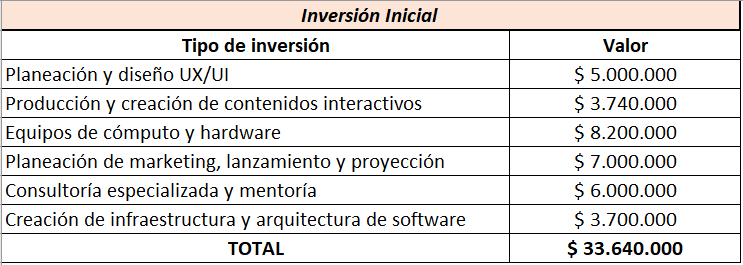
\includegraphics[width=12cm]{Imagenes/InversionInicial.png}
	\label{InversionInicial}
\end{table}